\documentclass[25pt, a0paper, portrait, margin=0mm, innermargin=20mm,
blockverticalspace=2mm, colspace=20mm, subcolspace=0mm]{tikzposter} %Default values for poster format options.

\input{packages}
\input{style}

\begin{document}

\renewcommand{\baselinestretch}{1}
\title{\parbox{1500pt}{Detection of transient communication signals in weakly electric fish}}
\author{Sina Prause, Alexander Wendt, and Patrick Weygoldt}
\institute{Supervised by Till Raab \& Jan Benda, Neuroethology Lab, University of Tuebingen}
\usetitlestyle[]{sampletitle}
\maketitle
\renewcommand{\baselinestretch}{1.4}

\begin{columns}
\column{0.4}
\myblock[TranspBlock]{Introduction}{
    The time-frequency tradeoff makes reliable signal detecion and simultaneous
    sender identification of freely interacting individuals impossible.
    This profoundly limits our current understanding of chirps to experiments
    with single - or physically separated - individuals.
    % \begin{tikzfigure}[]
    %     \label{griddrawing}
    %     \includegraphics[width=1\linewidth]{figs/introplot}
    % \end{tikzfigure}
}
\myblock[TranspBlock]{Chirp detection}{
    \begin{tikzfigure}[]
        \label{fig:example_a}
        \includegraphics[width=1\linewidth]{figs/algorithm}
    \end{tikzfigure}
    \vspace{0cm}
}

\column{0.6}
\myblock[TranspBlock]{Chirps during competition}{
    \begin{tikzfigure}[]
        \label{fig:example_b}
        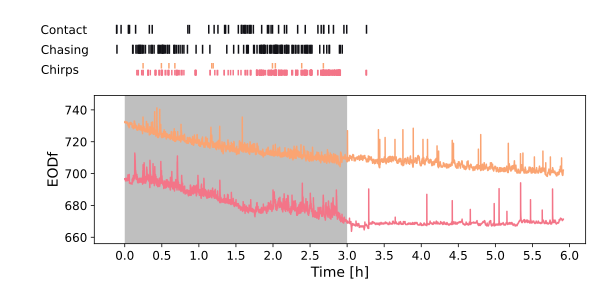
\includegraphics[width=\linewidth]{figs/timeline.pdf}
    \end{tikzfigure}
    \noindent
    \begin{tikzfigure}[]
        \label{fig:example_b}
        \includegraphics[width=\linewidth]{figs/chirps_winner_loser.pdf}
    \end{tikzfigure}
    \noindent
}

\myblock[TranspBlock]{Interactions at modulations}{
    \vspace{-1.2cm}
    \begin{tikzfigure}[]
        \label{fig:example_c}
        \includegraphics[width=0.5\linewidth]{example-image-c}
    \end{tikzfigure}

    \begin{multicols}{2}
        \begin{itemize}
            \setlength\itemsep{0.5em}
            \item $\Delta$EOD$f$ does not appear to decrease during synchronous modulations ().
            \item Individuals that rise their EOD$f$ first appear to rise their frequency higher compared to reactors (\textbf{B}).
            \vfill
            \null
            \columnbreak
            \item Synchronized fish keep distances below 1 m (\textbf{C}) but distances over 3 m also occur (see \textbf{movie}).
            \item Spatial interactions increase \textbf{after} the start of a synchronous modulation (\textbf{D}).
        \end{itemize}
    \end{multicols}
    \vspace{-1cm}
}

\myblock[GrayBlock]{Conclusion}{
    \begin{itemize}
        \setlength\itemsep{0.5em}
        \item Our analysis is the first to indicate that \textit{A. leptorhynchus} uses long, diffuse and synchronized EOD$f$ signals to communicate in addition to chirps and rises.
        \item The recorded fish do not exhibit jamming avoidance behavior while close during synchronous modulations.
        \item Synchronous signals \textbf{initiate} spatio-temporal interactions.
    \end{itemize}
    \vspace{0.2cm}
    }
    \end{columns}

\node [above right,
    text=white,
    outer sep=45pt,
    minimum width=\paperwidth,
    align=center,
    draw,
    fill=boxes,
    color=boxes] at (-43.6,-61) {
        \textcolor{white}{
    \normalsize Contact: \{name\}.\{surname\}@student.uni-tuebingen.de}};

\end{document}
